\documentclass[main.tex]{subfiles}
% 集合与映射
\begin{document}
集合是近代数学的基本语言。连续介质力学中的大量概念都依赖集合来定义。而集合本身却是难以借助更基础的概念进行定义的“最原始概念”。因此在下述集合的定义只能假定每一位读者都能一致地理解。
\begin{definition}[集合]
集合是具有某种特性的事物的整体。构成集合的事物或对象称为元素或成员。集合还必须满足:
\begin{itemize}
    \item 无序性:一个集合中,每个元素的地位是相同的,元素之间是无序的
    \item 互异性:一个集合中,任何两个元素都不相同,即每个元素只出现一次
    \item 确定性:给定一个集合及一个事物,该事物要么属于要么不属于该集合,不允许模棱两可。
\end{itemize}
\end{definition}

集合的表示方式有列举法和描述法。例:以下都是集合。
\begin{align*}
    A&=\{2,4,6,8\}\\
    B&=\{n|n\text{是偶数且}1<n<9\}\\
    1&\notin A, 2\in B
\end{align*}

我们能否说上例的两个集合是“相同”的或“相等”的?下一条定义将明确这一问题的答案。

\begin{definition}[子集、包含、集合的相等]
如果只要\(a\notin B\),则必有\(a\in A\),则称$B$是$A$的子集,或称$A$包含$B$,记为\(B\subseteq A\),\(A\supseteq B\)。如果\(A\subseteq B\)且\(B\subseteq A\)则称\(A=B\)。
\end{definition}

可验证如下定理:

\begin{theorem}
\begin{enumerate}
\item \(S\subseteq S, \forall S\),
\item 若\(A\subseteq B\)且\(B\subseteq C\)则\(A\subseteq C\)。
\end{enumerate}
\end{theorem}

\begin{definition}[真子集、真包含]
若\(B\subseteq A\)且\(B\neq A\),则称$B$是$A$的真子集,或称$A$真包含$B$,记为\(B\subset A\),\(A\supset B\)。
\end{definition}

可验证如下定理:
\begin{theorem}
\begin{enumerate}
    \item $\forall S$,$S\subset S$均不成立。
    \item 若$A\subset B$则$B\subset A$不成立。
    \item 若$A\subset B$且$B\subset C$,则$A\subset C$。
\end{enumerate}
\end{theorem}

\begin{definition}[空集]
空集$\emptyset = \{a|a\neq a\}$
\end{definition}

可验证如下定理:

\begin{theorem}
\begin{enumerate}
    \item $\emptyset\subseteq A,\forall A$。
    \item $\emptyset\subset A,\forall A\neq\emptyset$。
\end{enumerate}
\end{theorem}

\begin{definition}[并集]
若$a\in A$或$a\in B,\forall a,A,B$,则$a\in A\cup B$,称$A$与$B$的并集。
\end{definition}

可验证:
\begin{theorem}
并集关系具有以下性质:
\begin{enumerate}
    \item 结合律:$A\cup\left(B\cup C\right)=\left(A\cup B\right)\cup C$。
    \item 交换律:$A\cup B=B\cup A$。
    \item $\emptyset\cup A=A,\forall A$。
\end{enumerate}
\end{theorem}

\begin{definition}[交集]
若$a\in A$且$a\in B,\forall a,A,B$,则$a\in A\cap B$,称$A$与$B$的交集。
\end{definition}

\begin{definition}[笛卡尔积]
两个集合$A$和$B$的笛卡尔积是所有有序对$\left(a,b\right),a\in A,b\in B$的集合: $A\times B=\{\left(a,b\right)|a\in A\text{且}b\in B\}$
\end{definition}

我们可以推广这一定义至任意个集合的笛卡尔积。集合$A_1,A_2,\cdots,A_n$的笛卡尔积是$A_1\times A_2\times\cdots\times A_n=\left\{\left(a_1,a_2,\cdots,a_n\right)|a_i\in A_i\right\}$,一个有序$n$元组的集合。如果$A_1=A_1=\cdots=A_n=A$,则记$A_1\times A_2\times\cdots\times A_n=A^n$。例如,$\mathbb{R}$是实数集,$\mathbb{R}^n$是$n$元有序实数组的集合,在解析几何中常用以表示$n$维欧几里德空间中一个点的坐标。

一个集合的元素可以与另一个集合的元素建立对应关系。我们主要关心的是满足某种规定的对应关系,称为映射,定义如下。

\begin{figure}[htbp]
\centering
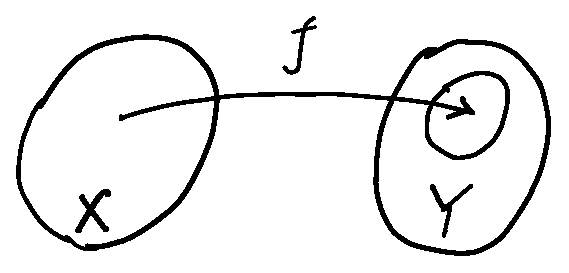
\includegraphics[width=0.25\textwidth]{images/II.1.1.eps}
\caption{映射}
\label{fig:II.1.1}
\end{figure}

\begin{definition}[映射]
(如图\ref{fig:II.1.1}所示)从集合$X$到集合$Y$的映射$f$,记为$f:X\rightarrow Y$,是$X$的所有元素与$Y$的部分或所有元素之间的对应关系,且每个$X$的元素只对应$Y$的一个元素。如果$y\in Y$是$x\in X$通过映射$f$的对应,则可写成:
\[y=f\left(x\right)\text{或}x\mapsto f\left(x\right)\text{或}f:x\mapsto y\]
并称$f\left(x\right)$是$x$的像。按上述定义,$x$只有一个像。$X$称为该映射$f$的定义域,记为$\mathrm{dom}f$,$Y$称为该映射$f$的陪域(codomain)或到达域(target domain)。$x$的像$f\left(x\right)$是$Y$的子集,称为该映射$f$的值域(range),记为$\mathrm{ran}f$。
\end{definition}

当映射的陪域是实数集$\mathbb{R}^n$或复数集$\mathbb{C}^n$时,我们常常也称其为函数。

\begin{definition}[映射的相等]
若映射$f:X\rightarrow Y$和$g:X\rightarrow Y$满足$f\left(x\right)=g\left(x\right),\forall x\in X$,则这两个映射相等。
\end{definition}

\begin{definition}[恒等映射]
恒等映射$\mathrm{id}_A:A\rightarrow A$是由集合$A$到其自身的映射:$\mathrm{id}_A\left(a\right)=a,\forall a\in A$。
\end{definition}

\begin{figure}[htbp]
\centering
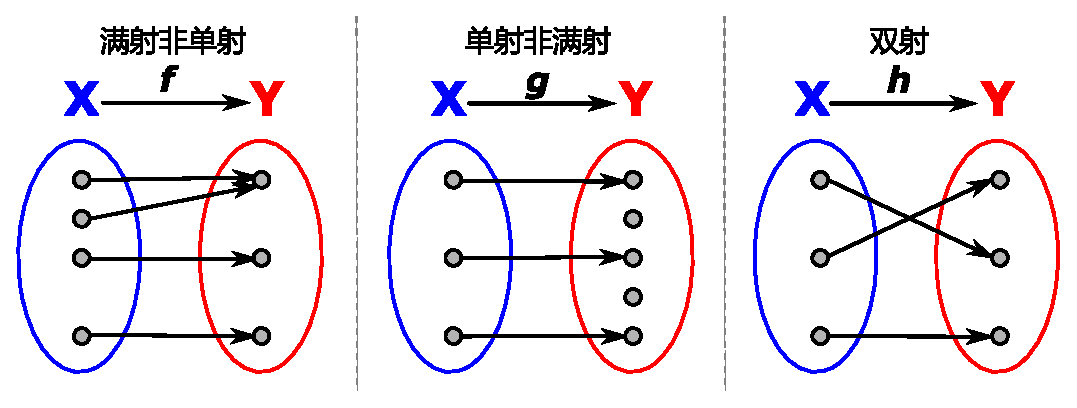
\includegraphics[width=0.5\textwidth]{images/II.1.2.eps}
\caption{满射、单射和双射}
\label{fig:II.1.2}
\end{figure}

\begin{definition}[单射、双射、满射]
(如图\ref{fig:II.1.2}所示)对于映射$f:X\rightarrow Y$,若$f\left(x_1\right)=f\left(x_2\right)\Rightarrow x_1=x_2$,则映射$f$是单射(injective mapping)。若$f\left(X\right)=Y$,则称$f$是满射(surjective mapping)。既是单射又是满射的映射叫双射(bijective mapping)。
\end{definition}

读者可自行画图表示非满射非单射的情况。

\begin{definition}[复合映射]
令$f:X\rightarrow Y$和$g:Y\rightarrow Z$是两个映射。则$f$和$g$的复合映射,记为$g\circ f$,是从$X$到$Z$的映射:
\[g\circ f\left(x\right)=g\left(f\left(x\right)\right),\forall x\in X\]
\end{definition}

\begin{theorem}
对于映射$f:X\rightarrow Y$和$g: Y\rightarrow Z$,
\begin{itemize}
    \item 如果$f$和$g$都是满射,则$g\circ f$是满射
    \item 如果$g\circ f$是满射,则$g$是满射
\end{itemize}
\end{theorem}
\begin{proof}
留作练习。
\end{proof}

\begin{theorem}
对于映射$f:X\rightarrow Y$和$g: Y\rightarrow Z$,
\begin{itemize}
    \item 如果$f$和$g$都是单射,则$g\circ f$是单射
    \item 如果$g\circ f$是满射,则$f$是单射
\end{itemize}
\end{theorem}
\begin{proof}
留作练习。
\end{proof}

\begin{definition}[逆映射]\label{def:II.1.14}
对于映射$f:X\rightarrow Y$,如果存在一个映射$g:Y\rightarrow X$,使得复合映射$g\circ f$是恒等映射$\mathrm{id}_X$,则称映射$f$是可逆的,映射$g$是$f$的逆映射。
\end{definition}

关于逆映射,有一条重要的定理,使得在今后的数学陈述和推理中,我们可以默认——
\begin{theorem}\label{thm:II.1.7}
双射必存在唯一逆映射。双射的逆映射也是双射。
\end{theorem}
\begin{proof}
为了证明这一定理,我们首先证明一个引理:任一单射非满射均存在逆映射。

设$f:X\rightarrow Y$是一个单射非满射,即$\exists y\notin\mathrm{f},y\in Y$。由集合的相关定义此处必有$\left\{y|y\in\mathrm{ran}f\right\}\cup\left\{y|y\notin\mathrm{ran}f,y\in Y\right\}=Y$。

现定义$g:Y\rightarrow X$,为使$g$为一个映射,它必须对$y\in\mathrm{ran}f$和$y\notin\mathrm{ran}f,y\in Y$均有定义。现将其定义为:
\[
g\left(y\right)=\left\{
\begin{array}{ll}
\left.x\right|_{f\left(x\right)=y},&y\in\mathrm{ran}f\\
\text{任一}x\in X,&y\notin\mathrm{ran}f,y\in Y
\end{array}
\right.
\]
则有如下几条结论:
\begin{enumerate}
    \item $g\left(y\right)$是映射。因为它对每一$y\in Y$均有定义且一个$y\in Y$只对应一个$x\in X$。
    \item $g$是满射。因为,仅$y\in\mathrm{ran}f$情况的定义式就已决定了$\mathrm{ran}g=X$。
    \item $g$是非单射。因为$g$是满射,再考虑$y\notin\mathrm{ran}f,y\in Y$情况的定义式,就可知$\exists x\in X$满足$x=g\left(y\right)=g\left(y^\prime\right)$,其中$y\neq y^\prime,y\in\mathrm{ran}f,y^\prime\notin\mathrm{ran}f,y^\prime\in Y$。
    \item $g$是$f$的逆映射。因为,对于任一$x\in X$均有$g\circ f\left(x\right)\equiv g\left(f\left(x\right)\right)=x$,即$g\circ f=\mathrm{id}_X$。
    \item 一般地,$g$是不唯一的。因为$y\notin\mathrm{f},y\in Y$的情况可定义$g\left(x\right)$等于任一$x\in X$,故只要集合$X$不是只有一个元素,那么$g$都不唯一。
\end{enumerate}
该引理证毕。

现在正式证定理\ref{thm:II.1.7}。从上面定义的这个$g$继续,如果$g$是双射,则$g$不仅是满射,还是单射。由刚刚证完的引理,可用类似方法给$g$找一个逆映射$f^\prime:X\rightarrow Y$。而且,由于$\mathrm{ran}g\equiv X$,我们无需像定义$g$那样为$f^\prime$分出$x\notin\mathrm{ran}g,x\in X$的情况,因为不存在这种情况。故
\[
f^\prime\left(x\right)=\left.y\right|_{g\left(y\right)=x}
\]
是$g$的逆映射,且$f^\prime$是满射。而且,把$g$的定义代入上式有$f^\prime\left(x\right)=\left.y\right|_{g\left(y\right)=x}=\left.y\right|_{\left.x\right|_{f\left(x\right)=y}}=f\left(x\right)$,即$f^\prime$不是别的映射而恰为$f\left(x\right)$。即$g$的逆映射是唯一的。因$f^\prime$是满射故$f$是满射,而$f$本身就是单射,故$f$是双射。
\end{proof}
\end{document}
